\datos{color}{}{}
\subsection{\textit{TurtleBot 4}}
%\addcontentsline{toc}{section}{Ejercicio 1}

\textit{TurtleBot 4}, Figura \ref{turtlebot4}, es una plataforma móvil educativa y de investigación 
desarrollada en 2022 por 
\textit{Clearpath Robotics} y \textit{Open Robotics}. Está construida sobre la base del robot
móvil \textit{iRobot Create 3}, que actúa como plataforma de locomoción y sensorización de bajo nivel.
Sobre esta base se integra un conjunto de sensores modernos, como un \textit{LiDAR} 2D, una 
cámara \textit{RGB-D}, una \textit{IMU} y un ordenador principal, \textit{Raspberry Pi 4B},
que ejecuta los módulos de percepción, \textit{SLAM}, navegación y 
control dentro del ecosistema \textit{ROS2} (\textit{Robot Operating System}). 
Gracias a esta combinación, el \textit{TurtleBot 4}
es uno de los robots más utilizados en universidades y laboratorios para la 
enseñanza y experimentación en robótica móvil, así como para el desarrollo de aplicaciones 
prototipo. \\

Sus usos principales abarcan la educación en robótica y \textit{ROS2}, la investigación
en navegación autónoma y el diseño de algoritmos de \textit{SLAM}, percepción y planificación. \\

\begin{wrapfigure}{r}{0.4\textwidth}
    \centering
    \vspace{-10pt}
    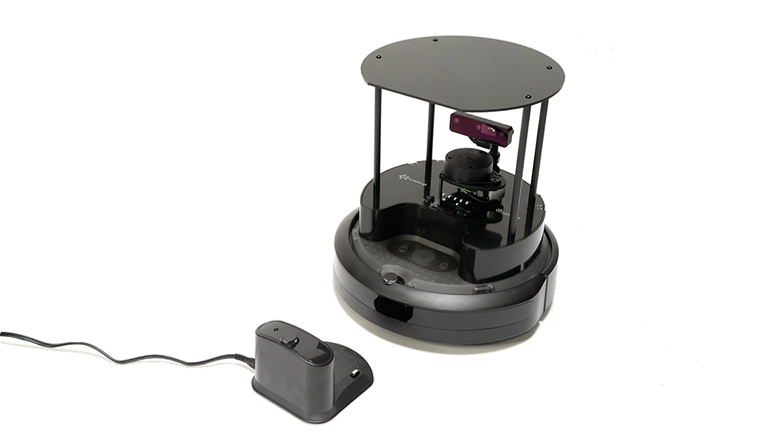
\includegraphics[width=0.4\textwidth]{Images/turtlebot.png}
    \caption{\textit{TurtleBot 4}.}
    \label{turtlebot4}
    \vspace{-10pt}
\end{wrapfigure}

Al igual que el robot \textit{Shakey}, el \textit{TurtleBot 4} presenta una arquitectura centralizada. 
Todos los sensores envían sus datos crudos a un único ordenador principal, encargado de ejecutar
los nodos de percepción, localización, construcción del mapa, planificación de rutas y control
del movimiento. La toma de decisiones se concentra en este módulo central, desde el que se 
envían directamente las órdenes a los actuadores. En consecuencia, no existe una distribución
de la inteligencia entre múltiples unidades de procesamiento, sino una estructura jerárquica
clásica basada en la secuencia percepción $\rightarrow$ planificación $\rightarrow$ acción. \\

Este robot también utiliza un sistema de locomoción diferencial compuesto por dos ruedas 
motrices laterales accionadas de manera independiente y una rueda libre trasera que 
proporciona estabilidad. Variando la velocidad relativa de las dos ruedas motrices, 
el robot puede avanzar, retroceder, girar sobre su eje y realizar maniobras precisas 
en entornos principalmente interiores.

\begin{comment}
\begin{figure}[H]
    \begin{center}
    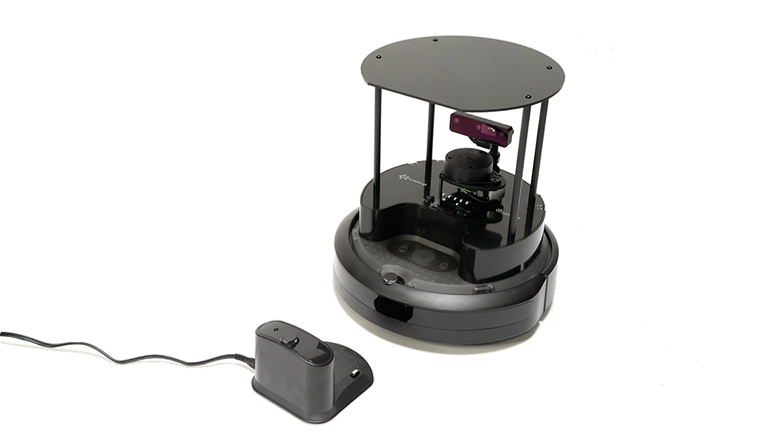
\includegraphics[scale=0.3]{Images/turtlebot.png}
    \caption{\textit{TurtleBot 4}.}
    \label{turtlebot4}
    \end{center}
\end{figure}
\end{comment}

\subsection*{Referencias}
\cite{TurtleBot4Clearpath} \fullcite{TurtleBot4Clearpath}.\\

\cite{TurtleBot4Manual} \fullcite{TurtleBot4Manual}.\\

\cite{iRobotCreate3} \fullcite{iRobotCreate3}.
